\documentclass[aspectratio=169, ignorenonframetext]{beamer}
\usepackage{pgf}

\mode<article>{
  \usepackage{fullpage}

}

\mode<presentation>
{
  \usetheme{Madrid}
  \useinnertheme{circles}
  \setbeamertemplate{navigation symbols}{}
%   \usetheme[hideothersubsections, width=2.4cm]{Hannover}
%   \usetheme{Antibes}
%   \usetheme{Montpellier}
%   \usetheme{Singapore}
%   \usecolortheme{seahorse}
   \setbeamertemplate{footline}
   {%
%      \begin{beamercolorbox}{section in head/foot}
%       \usebeamercolor{bg}
%        \hskip 1em \footnotesize \insertframenumber{} / \inserttotalframenumber%\hskip 41em 
\includegraphics[height = .5cm]{../../bilder/cc_by-nc_eu.png}
%        
\includegraphics{../../bilder/cc_by-nc_eu.png}
% cc_by-nc_eu.png: 403x141 px, 72dpi, 14.22x4.97 cm, bb=0 0 403 141

% % cc_by-nc_eu.png: 403x141 px, 72dpi, 14.22x4.97 cm, bb=0 0 403 141
%
% % bwslogo_3.png: 476x392 px, 300dpi, 4.03x3.32 cm, bb=0 0 114 94
%
%       %\hskip 5em
%       %       \input{../bilder/cc_by.png}
%       %\includegraphics[height=.5cm]{../../../../bilder/bwslogo_3.png}
%      \end{beamercolorbox}%
   }
  \usepackage{beamerfoils}
}
\usepackage[utf8]{inputenc}
\usepackage[german]{babel}
\usepackage[utf8]{inputenc}
\usepackage{times}
\usepackage[T1]{fontenc}
\usepackage{eurosym}
\usepackage{graphicx}
\usepackage{amsmath}
\usepackage[siunitx,european]{circuitikz}
% \usepackage{ulem}
\usepackage{listings}
%
\lstset{numbers=left, numberstyle=\tiny, stepnumber=2, numbersep=5pt, language = C++, alsolanguage=XML}

\only<article>{
  \usepackage[colorlinks=true,linkcolor=blue,filecolor=magenta,urlcolor=cyan]{hyperref}
}

\only<presentation>{
\MyLogo{\includegraphics[height=1cm]{../../../../../bilder/bwslogo_3.png}}
  \usepackage{hyperref}
}


\title{Arbeitsunterlagen zu FOS Elektrotechnik Themenfeld 12.4}
\subtitle{}
% \date{Stand: \today}%\\

\institute[BWS Hofheim]{Brühlwiesenschule, Hofheim}
\author{Thomas Maul}

\titlegraphic{Für eigene Teile gilt: 
\includegraphics[height=1cm]{../../bilder/cc_by-nc_eu.png}}


\begin{document}

  \only<article>{
    \maketitle
    \tableofcontents
    \clearpage
  }
\begin{frame}<beamer>
  \titlepage
  % \hyperlink{Teil_2}{\beamerbutton{Go part 2}}
\end{frame}

\begin{frame}{Diode}
  \begin{itemize}
    \item Halbleiter (oft Silizium)
    \item Einweg-Durchlass
    \item Spannungsverlust = Durchbruchspannung
    \item begrenzter Strom
  \end{itemize}
\end{frame}

\begin{frame}{Aufgabe}
  \begin{itemize}
    \item Versorgung einer elektronischen Schaltung
    \item 5V =
    \item Versorgung: 12V $\approx$
    \pause
    \item "`Du kannst das doch :)"'
  \end{itemize}
\end{frame}

\begin{frame}{Bilder}
  \begin{columns}
   \begin{column}{.5\textwidth}
 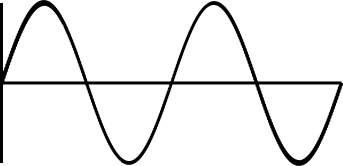
\includegraphics[scale=0.7]{sinuswelle.png}
 "`vorher"'
   \end{column}
   \begin{column}{.5\textwidth}
    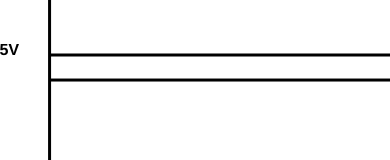
\includegraphics[scale=.7]{gleichspannung5v.png}
    nachher (Ziel)
   \end{column}
  \end{columns}
\end{frame}

\begin{frame}{Lösung (1)}
  \begin{columns}
    \begin{column}{.5\textwidth}
      \begin{itemize}
        \item <1->Diode als Gleichrichter "`Einweg-Gleichrichter"'
        \item <1->Pulsierende Gleichspannung (50\% der Zeit = 0 V)
        \item <2->Glättung mit Kondensator (C ist parallel zu Last/Verbraucher) $\text{R}_v$ nicht vergessen
      \end{itemize}
   \end{column}
   \begin{column}{.5\textwidth}
     \only<1>{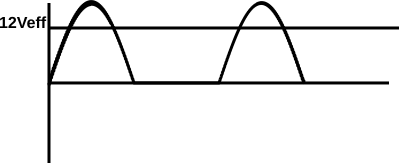
\includegraphics[scale=0.7]{sinuswelleGleichrichter_12v.png}}
     \only<2>{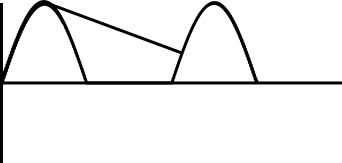
\includegraphics[scale=0.7]{sinuswelleGleichrichter_glaettung1.png}}
   \end{column}
  \end{columns}
\end{frame}

\begin{frame}{Lösung (2)}
  \begin{columns}
    \begin{column}{.5\textwidth}
      \begin{itemize}
        \item <1->4 Dioden als Gleichrichter "`Brücken-Gleichrichter"'
        \item <1->Pulsierende Gleichspannung
        \item <2->Glättung mit Kondensator (C ist parallel zu Last/Verbraucher) $\text{R}_v$ nicht vergessen
      \end{itemize}
   \end{column}
   \begin{column}{.5\textwidth}
     \only<1>{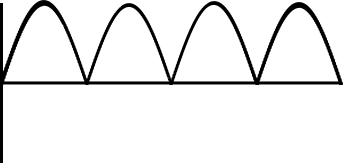
\includegraphics[scale=0.7]{sinuswelleGleichrichterBruecke.png}}
     \only<2>{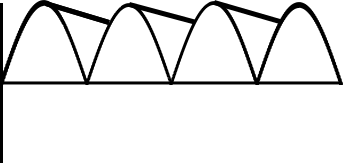
\includegraphics[scale=0.7]{sinuswelleGleichrichterBrueckeGlaettung}}
   \end{column}
  \end{columns}
\end{frame}

\begin{frame}{Aufgaben}
  \begin{itemize}
    \item informiere dich über die Strompfade bei m Brückengleichrichter.
    \item Informiere dich über die Glättungsschaltung (mit Kondensator).
    \item Wie groß muss ein C sein für Eingang 12V (2 A), Verbraucher 5\,V, 500 mA.
    \item Welche Diode(n) benötige ich für die Gleichrichtung (Typ z. B. 1N4148).
  \end{itemize}
\end{frame}

\end{document}
